En esta sección se diseñan dos algoritmos que buscan resolver el problema de la distancia mínima de edición extendida entre dos cadenas dadas, S1 y S2. Cada algoritmo utiliza las operaciones de inserción, sustitución, eliminación, y la variante de transposición, junto con sus respectivos costos.

El primer enfoque, \textit{"Fuerza Bruta"}, implementa una solución exhaustiva en la que se exploran todos los caminos posibles para transformar S1 en S2. En este enfoque, para hacer coincidir un solo carácter entre ambas cadenas, se generan todas las opciones posibles, lo que crea un árbol de decisiones donde cada nodo representa una operación. A medida que se avanza en cada carácter de las cadenas, el proceso se repite recursivamente para las letras restantes, evaluando todas las combinaciones de operaciones posibles. Al final, cuando se han recorrido todas las ramas del árbol, se selecciona la solución con el menor costo total.

Por ejemplo, consideremos las palabras S1 = 'amores' y S2 = 'amaras'. Al comparar los primeros caracteres de ambas cadenas, no se genera ningún conflicto; sin embargo, al llegar al tercer carácter de S1 'o' y compararlo con el tercer carácter de S2 'a', el algoritmo calcula los costos de las cuatro posibles operaciones (inserción, eliminación, sustitución y transposición) para hacer que ambos caracteres coincidan. Cada una de estas operaciones genera una llamada recursiva para el resto de la cadena, resultando en cuatro ramificaciones desde este punto en el árbol.

Este proceso continúa a medida que avanzamos en las cadenas, y al comparar el quinto carácter de S1 'e' con el quinto de S2 'a', cada una de las cuatro ramificaciones previas vuelve a generar otras cuatro, ya que cada rama evalúa nuevamente las cuatro operaciones posibles. Esto resulta en un árbol de decisiones con 16 nodos hoja hasta este punto.

Este proceso puede visualizarse más fácilmente en el siguiente diagrama del árbol resultante, que ilustra el crecimiento exponencial de las llamadas recursivas en el enfoque de Fuerza Bruta:
 
 \begin{minipage}[t]{0.5\textwidth}
    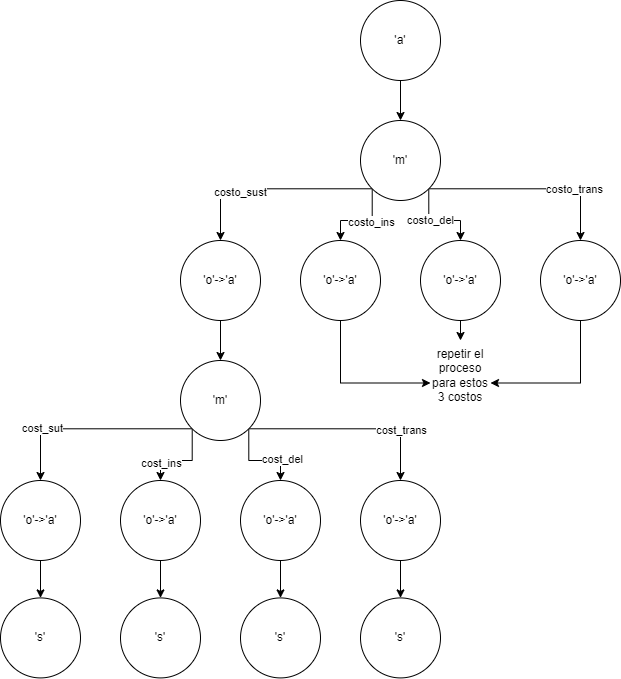
\includegraphics[width=\textwidth]{images/ejemplo_fuerza_bruta.png}
 \end{minipage}

 \begin{itemize}
     \item \textbf{Análisis Temporal}
     
     El análisis temporal del algoritmo de Fuerza Bruta, en el peor de los casos, considera que se deben calcular los costos para cada carácter de la cadena S1. A medida que se avanza en cada carácter, se generan cuatro ramificaciones (una para cada operación: inserción, eliminación, sustitución y transposición), lo cual expande exponencialmente el árbol de decisiones. Si consideramos que la longitud de S1 es \( n \), entonces el árbol resultante tendrá aproximadamente \( 4^n \) nodos en el peor de los casos, dado que cada operación genera cuatro posibles caminos a seguir. Por lo tanto, la complejidad temporal del algoritmo es \( O(4^n) \), lo que lo convierte en un método ineficiente para cadenas largas debido a su crecimiento exponencial en tiempo de ejecución.

    \item \textbf{Análisis Espacial}

    En cuanto al análisis espacial, la cantidad de espacio requerida difiere del crecimiento temporal. En el algoritmo de Fuerza Bruta, cada llamada recursiva crea una copia de las cadenas restantes en la pila de ejecución, pero el almacenamiento de datos solo requiere guardar los caracteres de S1 y S2 en el nivel actual de la recursión. Esto significa que, en el primer nivel (la raíz del árbol de decisiones), se necesita espacio para \( n \) caracteres. A medida que se desciende en el árbol y se realizan llamadas recursivas, el espacio utilizado por cada nivel se reduce, ya que las cadenas a comparar disminuyen en tamaño. 

    Por lo tanto, en el último nivel, correspondiente a los nodos hoja, se almacenan únicamente las operaciones finales sobre caracteres individuales. Esto implica que el espacio máximo en la pila de ejecución está limitado por la profundidad del árbol, que es \( n \), resultando en una complejidad espacial de \( O(n) \).

 \end{itemize}